% ============================
\chapter{Les types}
\label{chap:types}
\index{type référénce}
\index{type primitif}
% ============================

\begin{Exergue}

	«~Un \pc{type} qui se trompe en disant quelque chose de faux dit peut-être
	quelque chose de vrai.~»

	\begin{flushright}

		Philippe Geluck
		
	\end{flushright}

\end{Exergue}

En langage Java, toute donnée à un type. 

Les données manipulées dans un programme peuvent être écrites dans le code du
programme ou être mémorisées le temps de l'exécution de celui-ci ou encore être
une entrée du programme. 


\marginicon{definition}
\begin{itemize}
	\index{littéral}
	\item Une valeur écrite dans un programme est appelée
		«~\textit{littéral}~». Cette valeur une valeur et un type. 

	\item Pour qu'une valeur soit mémorisée le temps de l'exécution —~ou tout
		du moins pendant une partie de l'exécution~— elle doit être stockée
		dans une variable (voir section \vref{primitif-reference}). Une
		variable a une valeur \textit{variable} et un type. 

\end{itemize}

\minitoc

\index{type primitif}
\section{Les types primitifs}

Il existe, en Java, 8 types primitifs~: des types primitifs numériques
entiers, numériques à virgule flottante, les  caractères et les booléens.
Voici ce que dit la grammaire~: 

\begin{grammaire}
	\grammarrule{PrimitiveType:}
		\grammarrule{NumericType}
		boolean

	\grammarrule{NumericType:}
		\grammarrule{IntegralType}
		\grammarrule{FloatingPointType}

	\grammarrule{IntegralType:}
		\grammarrule{(one of)}
		byte short int long char

	\grammarrule{FloatingPointType:}
		\grammarrule{(one of)}
		float double
\end{grammaire}

Chaque type a une taille déterminée. 

La figure \vref{fig:typesprimitifs} représente tous les types primitifs en
Java. Voyons les en détails.

\begin{figure}[h]
	\centering
	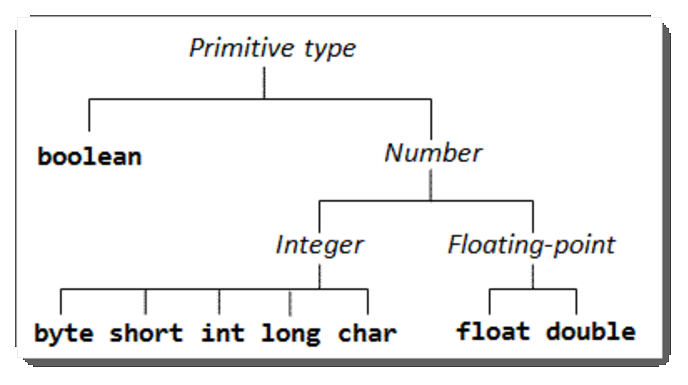
\includegraphics[width=.7\linewidth]{images/primitifs.pdf}
	\caption{Les types primitifs Java}
	\label{fig:typesprimitifs}
\end{figure}

\subsection{Les types primitifs numériques entiers}

Il existe 5 types primitifs entiers. Les 4 premiers représentent des nombres
entiers signés codés en notation en complément à 2. Il s'agit des types
: \pc{\bf byte}, \pc{\bf short}, \pc{\bf int} et \pc{\bf long}. 


La quantité mathématique montrée à la figure \vref{fig:7doigts} peut être
représentée de différentes manières : en utilisant des chiffres romains —~VII~—
ou arabes en base 10 —~7~— ou en base 2 —~111~— ou encore de moult autres
façons. 

Pour représenter un nombre négatif, l'habitude est de l'affubler du signe '-'
devant mais il est également possible d'utiliser la notation en complément à 2. 

\index{byte}
\index{short}
\index{int}
\index{long}
Les types \pc{byte}, \pc{short}, \pc{int} et \pc{long} représentent une partie
des nombres entiers signés. Ils sont stockés en notation en complément à 2. Ils
se différencient par la taille qu'ils occupent en mémoire et donc par
l'intervalle de nombres qu'ils représentent. 

La figure \vref{fig:typesbyteshortintlong} rassemble les types primitifs
entiers (excepté \pc{char}) avec leurs intervalles. 

\begin{figure}[h]
	\centering
	\begin{tabular}[h]{|l|l|p{9cm}|}
		\hline
		\rowcolor{black!20}
		\textbf{Type}	&	\textbf{Taille}	&	\textbf{Intervalle}	\\
		\hline
		\pc{byte}	&	8 bits	&	[-128, 127]\\
				&			&	[$-2^7$, $2^7-1$]\\
		\pc{short}	&	16 bits	&	[-32\,768-, 32\,767]\\
				&			&	[$-2^{15}$, $2^{15}-1$]\\
		\pc{int}		&	32 bits	&	[-2\,147\,483\,648, 2\,147\,483\,647]\\
				&			&	[$-2^{31}$, $2^{31}-1$]\\
		\pc{long}	&	64 bits	
			&	[-9\,223\,372\,036\,854\,775\,808, 9\,223\,372\,036\,854\,775\,807]\\
				&			&	[$-2^{63}$, $2^{63}-1$]\\
		\hline
	\end{tabular}	
	\caption{Types primitifs entiers (exceptés \pc{char}) et leur taille}
	\label{fig:typesbyteshortintlong}
\end{figure}

Le type \pc{int} est le type numérique entier privilégié. C'est celui qui est
le plus utilisé et est le type par défaut dans les opérations mathématiques
usuelles. L'intervalle qu'il représente est généralement suffisant%
\footnote{Ce qui n'est pas toujours vrai puisqu'en décembre 2014, la vidéo \textit{Gangnam Style} est la première vidéo Youtube à dépasser ±2 milliard de vues (2\,147\,483\,647 pour être précis) et oblique Google à revoir la variable dans laquelle elle stocke ce nombre de vues pour passer à 64 bits.}. 

\begin{figure}[h]
	\centering
	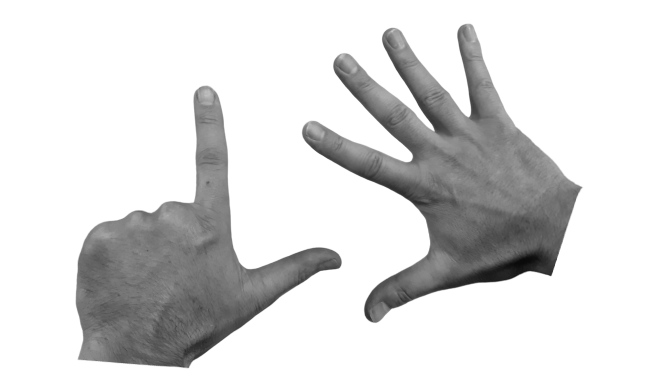
\includegraphics[width=.8\linewidth]{images/7doigts.png}
	\caption{La quantité 7 montrée avec les doigts}
	\label{fig:7doigts}
\end{figure}

\subsection{Les littéraux numérique entiers (excepté \pc{char})}

Les nombres entiers sont représentés en utilisant les chiffres habituels. Il
est cependant possible d'écrire un nombre dans différentes bases. Il faudra
alors pouvoir les distinguer. En mathématiques il est d'habitude d'utiliser un
indice pour préciser la base comme : $7_{10} = 111_2$. En informatique nous
utiliseront un \textbf{préfixe}. 

\textbf{Littéral numérique décimal}

Respecte les règles suivantes~:

\begin{itemize}
	\item les chiffres \texttt{0123456789} et \texttt{\_};
	\item un littéral est de type \pc{int} ou \pc{long}, jamais de type 
		\pc{byte} ou \pc{short}\footnote{Ceci ne nous empêchera pas d'écrire 
		\pc{byte b = 5} par exemple. Nous verrons les conversions en 
		Développement II};
	\item pour distinguer un littéral \pc{long} d'un \pc{int}, suffixer 
		d'un \texttt{l} ou \texttt{L};
\end{itemize}

\textit{Exemple, la quantité 100: }
\begin{java}
	int myInt = 100;
	int myOtherIntSomeValue = 1_00;
	long myLong = 100L;
\end{java}

\textbf{Littéral numérique octal}

Respecte les règles suivantes~:

\begin{itemize}
	\item les chiffres \texttt{01234567} et \texttt{\_};
	\item commence par un \texttt{0};
	\item un littéral est de type \pc{int} ou \pc{long}, jamais de type 
		\pc{byte} ou \pc{short};
	\item pour distinguer un littéral \pc{long} d'un \pc{int}, suffixer 
		d'un \texttt{l} ou \texttt{L};
\end{itemize}

\textit{Exemple, la quantité 100: }
\begin{java}
	int myOctalInt = 0144;
	int anoherOctalInt = 01_44;
	long myOctalLong = 0144L;
\end{java}

\textbf{Littéral numérique hexadécimal}

Respecte les règles suivantes~:

\begin{itemize}
	\item les chiffres \texttt{0123456789ABCDEFabcdef} et \texttt{\_};
	\item commence par un \texttt{0x} ou \texttt{OX};
	\item un littéral est de type \pc{int} ou \pc{long}, jamais de type 
		\pc{byte} ou \pc{short};
	\item pour distinguer un littéral \pc{long} d'un \pc{int}, suffixer 
		d'un \texttt{l} ou \texttt{L};
\end{itemize}

\textit{Exemple, la quantité 100: }
\begin{java}
	int myHexadecimalInt = 0x64;
	long myHexadecimalLong = 0X64l;
\end{java}

\textbf{Littéral numérique binaire}

Respecte les règles suivantes~:

\begin{itemize}
	\item les chiffres \texttt{01} et \texttt{\_};
	\item commence par un \texttt{0b} ou \texttt{OB};
	\item un littéral est de type \pc{int} ou \pc{long}, jamais de type 
		\pc{byte} ou \pc{short};
	\item pour distinguer un littéral \pc{long} d'un \pc{int}, suffixer 
		d'un \texttt{l} ou \texttt{L};
\end{itemize}

\textit{Exemple, la quantité 100: } 
\begin{java}
	int myBinaryInt = 0b01100100;
	int anotherBinaryInt = 0B0110\_0100;
\end{java}

\subsection{Le type primitif numérique entier particulier \pc{char}}

Le type \pc{char} est un entier non signé de 16~bits représentant le code 
Unicode codé en UTF-16 du caractère
	\footnote{%	
		Pour en savoir plus sur l'Unicode, UTF8, UTF16 et UTF32, lire
		«~Unicode, UTF8, UTF16, UTF32\ldots et tutti quanti~» \cite{pbt-unicode}
	}. 
Un caractère Unicode codé en UTF-16 fait une taille de 16 bits ou de 32 bits en
fonction du caractère qu'il représente. Le type \pc{char} en Java ne permet de
ne représenter que le sous ensemble BMP (\textit{Basic Multilingual Plane}) des
caractères Unicodes codés en UTF-16. Ceux ayant leur code compris entre
\texttt{\textbackslash u0000} et \texttt{\textbackslash uffff}. La figure 
\vref{fig:tableunicode} montre quelques caractères et leurs code Unicode. 

\begin{figure}[h]
	\centering
	\begin{tabular}[h]{|l|l|p{9cm}|}
		\hline
		\rowcolor{black!20}
		\textbf{Type}	&	\textbf{Taille}	&	\textbf{Intervalle}	\\
		\hline
		\pc{char}	&	16 bits	&	[0, 65\,535]\\
		&			&	[$0$, $2^{16}-1$]\\
		\hline
	\end{tabular}	
	\caption{Type primitif entier \pc{char} et sa taille}
	\label{fig:typeschar}
\end{figure}

\begin{figure}[t]
	\centering
	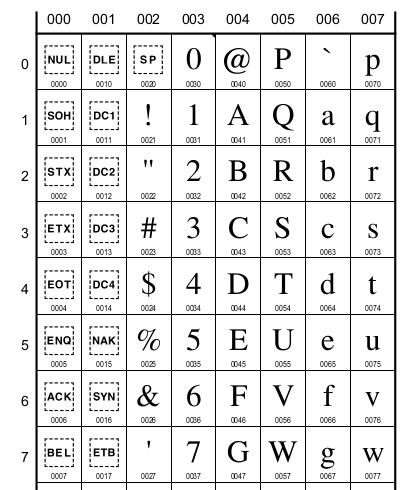
\includegraphics[width=.75\linewidth]{../images/unicode-latin.png}
	\caption{Extrait de la table Unicode \textit{Basic Latin (ASCII)}}
	\label{fig:tableunicode}
\end{figure}

\subsection{Les littéraux numériques entiers \pc{char}}

Un littéral de type \pc{char} se caractérise par les guillemets simples
(\textit{single quote}) qui l'entourent. 

Le caractère \textit{a} par exemple, se représente \texttt{'a'}. Et l'on pourra
déclarer une variable de type \pc{char} et l'initialiser avec le caractère
\textit{a} par une instruction de la forme~:

\begin{java}
	char myChar = 'a';
\end{java}

La variable \pc{myChar} de type \pc{char} est initialisée avec le littéral
\pc{'a'} de type \pc{char} également. 

\marginicon{definition}
\index{séquence d'échappement}
À ceci s'ajoute la possibilité \textbf{d'échapper des caractères}. Un caractère
peut parfois avoir plusieurs significations. Par exemple le caractère
\textit{single quote} (\pc{'}) signale le début d'un littéral de type \pc{char}
mais peut vouloir signaler simplement le caractère \pc{'}.   
Comment distinguer les deux ?

Lorsque l'on écrit simplement un caractère, il a sa signification habituelle~: 
\texttt{a} signifie \textit{a},
\texttt{b} signifie \textit{b},
\texttt{Z} signifie \textit{Z},
\texttt{'} signifie \textit{voici le début ou la fin d'un caractère}, etc. 
Certains caractères ont un \textbf{deuxième sens} lorsque qu'ils sont 
\textit{échappés}, c'est-à-dire précédés d'un \textit{backslash} 
(\pc{\textbackslash}). En voici quelques-uns~:

\begin{figure}[h]
	\centering
	\begin{tabular}[h]{|l|l|l|}
		\hline
		\rowcolor{black!20}
		\textbf{Caractère}	&	\textbf{Sens premier}	& \textbf{Sens second}	\\
		\hline
		n					&	n						& passage à la ligne	\\
		t					&	t						& tabulation		\\
		'					&	début ou fin d'un littéral \pc{char}	
														&	'	\\
		"					& 	début ou fin d'une chaine 	
														&	"	\\
		\hline
	\end{tabular}
	\caption{Quelques séquences d'échappement}
	\label{tab:séquenceséchappements}
\end{figure}



\subsection{Les types primitifs numériques à virgule flottante}

Les nombres pseudo-réels, ou encore les nombres à virgule flottante, sont un
sous ensemble des réels parce que —\,comme pour les entiers\,— il y aura un
\textit{plus petit nombre représentable} et \textit{un plus grand}. C'est
l'\textbf{intervalle} de nombre que l'on peut représenter. À ceci, s'ajoute la
\textbf{précision} que l'on pourra atteindre. En effet, les réels est un
ensemble continu de nombre —\,entre deux nombre réels, il existe toujours, au
moins, un autre réel\,— tandis que les pseudo-reéls est un ensemble discret. 

Les nombres à virgule flottante (\textit{floating numbers}) sont codés suivant
la norme \href{https://fr.wikipedia.org/wiki/IEEE_754}{IEEE\,754}. 

Selon cette norme, un nombre est représenté avec un signe, une mantisse et un
exposant. Le tout en base 2. Un bit est utilisé pour le signe.  

\[
	nombre = signe~mantisse_2~2^{exposant_2} 
\]

Il existe 2 types primitifs à virgule flottante~: \textbf{\texttt{float}} et
\textbf{\texttt{double}}.

\begin{figure}[h]
	\centering
	\begin{tabular}[t]{|l|c|c|c|}
		\hline
		\rowcolor{black!40}
		\textbf{Type} 	& \textbf{Taille (\textit{bit})}	
								& \textbf{Exposant} & \textbf{Mantisse}\\
		\hline
		float	& 32 bits					& 8		& 23\\
		\hline
		double	& 64 bits					& 11	& 52\\
		\hline
	\end{tabular}
	\caption{Types primitifs numériques à virgule flottante et leur taille}
	\label{fig:typefloat}
\end{figure}



\subsection{Les littéraux numériques à virgule flottante}

Les littéraux à virgule flottante sont composés de plusieurs parties~: une
partie entière, un point décimal (ou hexadécimal), une partie décimale, un
exposant et un suffixe.

\bigskip
\begin{center}
	\large\bf	| partie entière | . | partie décimale | exposant | suffixe |
\end{center}
\bigskip

Un littéral à virgule flottante peut être exprimé en base 10 (décimal) ou en 
base 16 (hexadécimal). 

Un littéral à virgule flottante est de type \pc{float} s'il est suffixé d'un
\pc{f} ou \pc{F} sinon, il est de type \pc{double}. Et ce qu'il soit suffixé
d'un \pc{d} ou \pc{D} ou non. 

Pour un \textbf{littéral décimal à virgule flottante}, au minimum un chiffre
dans la partie entière ou décimale et soit le point décimal, soit l'exposant,
soit le suffixe sont requis. Les autres parties sont optionnelles. 

\begin{itemize}

	\item la partie entière et la partie décimale sont des littéraux décimaux
		entiers (le caractère \pc{\_} étant autorisé);

	\item le point décimal est un point (\pc{.});

	\item l'exposant est la lettre \pc{e} ou \pc{E} suivie par un littéral
		décimal entier (le caractère \pc{\_} étant autorisé);

	\item le suffixe est \pc{f}, \pc{F}, \pc{d} ou \pc{D}

\end{itemize}

\textit{Exemples:}
\begin{java}
	double myDouble;
	myDouble = 1.;			// 1.0
	myDouble = .1;			// 0.1
	myDouble = 1e1;			// 10.0
	myDouble = 1d;			// 1.0
	myDouble = 1.e0;		// 1.0
	myDouble = 1_000.45;	// 1000.45
	myDouble = 1.45e3;		// 1450.0
	myDouble = .45e3d;		// 450.0
	
	float myFloat;
	myFloat = 1f;			// 1.0
	myFloat = 1.f			// 1.0	
\end{java}

Pour un \textbf{littéral hexadécimal à virgule flottante}, au minimum un
chiffre dans la partie entière ou décimale et l'exposant sont obligatoires. Le
suffixe est optionnel. 

\begin{itemize}

	\item le littéral débute par \pc{0x} ou \pc{0X};

	\item la partie entière et la partie décimale sont des chiffres hexadécimaux
		(le caractère \pc{\_} étant autorisé);

	\item le point décimal est un point (\pc{.});

	\item l'exposant est la lettre \pc{p} ou \pc{P} suivie par un littéral
		décimal entier (le caractère \pc{\_} étant autorisé) représentant une 
		puissance de 2;

	\item le suffixe est \pc{f}, \pc{F}, \pc{d} ou \pc{D}

\end{itemize}

\textit{Exemples:}
\begin{java}
	double myDouble;
	myDouble = 0x1p0;		// 1.0 = 1 * 2^0
	myDouble = 0x1.1p0;	// 1.0625 = 1 + (1/16)
	myDouble = 0x1p1;		// 2.0 = 1 * 2^1
	myDouble = 0xA.Bp0; // 10.6875= 10 + 11*1/16
	myDouble = 0x1E2p2; // 1928 = (1*16^2 + 14*16^1 + 2*16^0) * 2^2

	float myFloat;
	myFloat = 0X.1p4f;		// 1.0 = (1*16^-1) * 2^4

\end{java}




\subsection{Le type primitif booléen}

Le type primitif booléen permet de représenter les deux valeurs logiques
\textit{vrai} et \textit{faux}. Ce sont les deux seules valeurs de ce types. 


\subsection{Les littéraux booléens}

Les littéraux booléens sont simplement~: \pc{true} pour \textit{vrai} et
\pc{false} pour \textit{faux}. 

\textit{Exemple:}
\begin{java}
	boolean myBoolean = true;
\end{java}










\index{type référénce}
\section{Les types références}
